\subsection{Gain Scheduling}
    Bei nichtlinearen Systemen will man meist um verschiedene Betriebspunkte linearisieren. Dafür braucht es bei jedem Betriebspunkt einen anderen linearen Regler. Bei einem PI-Regler werden $k_p(o),\, T_i(o)$ zu Funktionen des Betriebspunktes $o$.
    
    \begin{figure}[H]
        \centering
        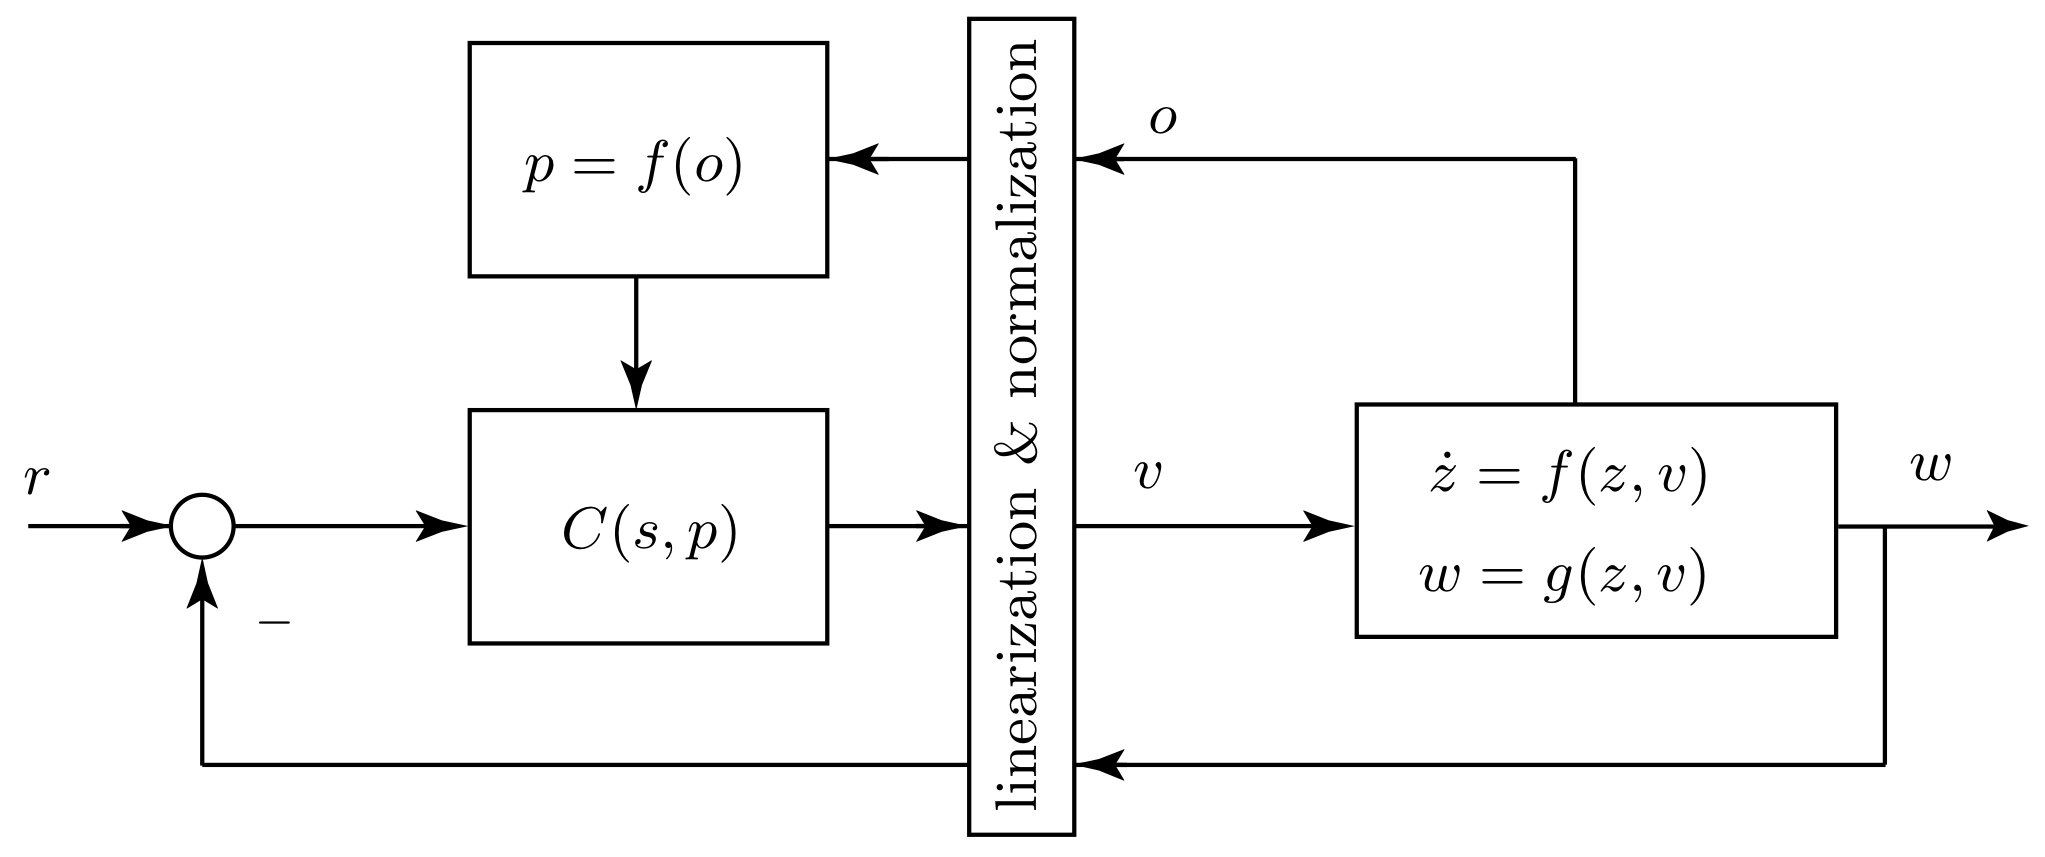
\includegraphics[width = 0.8\linewidth]{images/04/gain_sched.jpeg}
        \caption{Diagramm zu Gain scheduling}
    \end{figure}
    
\subsection{Analoge Realisierung}
    In manchen Anwendungen macht es Sinn, den Regler durch analoge Schaltungen anstatt durch Software zu realisieren. Mit diesen kann man eine Eingangsspannung $U_e$ in eine Ausgangsspannung $U_a$ umwandeln. Dabei kann man folgender Grundstruktur folgen:
    
    \begin{figure}[H]
        \centering
        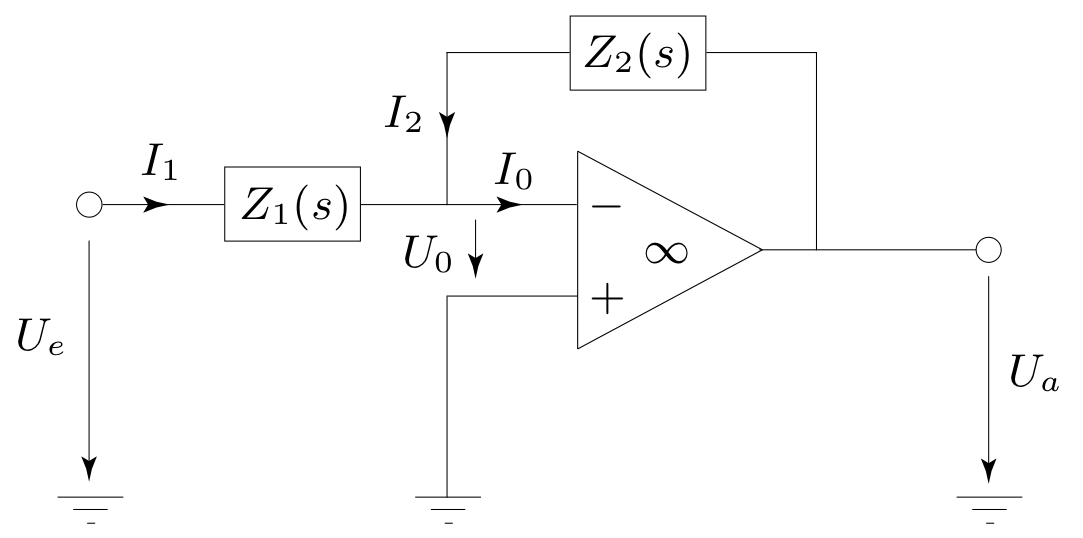
\includegraphics[width = 0.8\linewidth]{images/04/analog_real.jpeg}
        \caption{Grundstruktur analoge Realisierung mit einem idealen Op-Amp}
    \end{figure}
    
    Die Übertragungsfunktion lautet dabei
    \begin{equation*}
        \Sigma(s) = \frac{U_a(s)}{U_e(s)} = -\frac{Z_2(s)}{Z_1(s)}
    \end{equation*}
    
    Dabei konstruiert man $Z_1(s),\, Z_2(s)$ aus Widerständen ($R$), Induktoren ($L$) und Kapazitäten ($C$)
    \begin{equation*}
        Z_r(s) = R, \qquad Z_L(s) = s\cdot L, \qquad Z_c(s) = \frac{1}{s\cdot C}
    \end{equation*}
    
    Die Kirchhoffschen Reglen für Serie- und Parallelschaltungen von Elementen helfen bei der Realisierung der TF.
    
\subsection{Zeitdiskrete Realisierung}
    Da ein Regler, der auf Software basiert nur bei einer fixen Taktfrequenz $\mathit{f}_s$ an diskreten Stellen den Regel auswerten kann, muss man einen continuous-time Regler $C(s)$ ind einen discrete-time Regeler $C(z)$ umwandeln. Es können nur an fixen Zeitpunkten $t_n$ neue eingänge $u(n\cdot T_s):=u[k]$ berechnet werden:
    \begin{equation*}
        t_n = \frac{n}{\mathit{f}_s} = n\cdot T_s,\, n\in0,1,\dots
    \end{equation*}
    
    \begin{figure}[H]
        \centering
        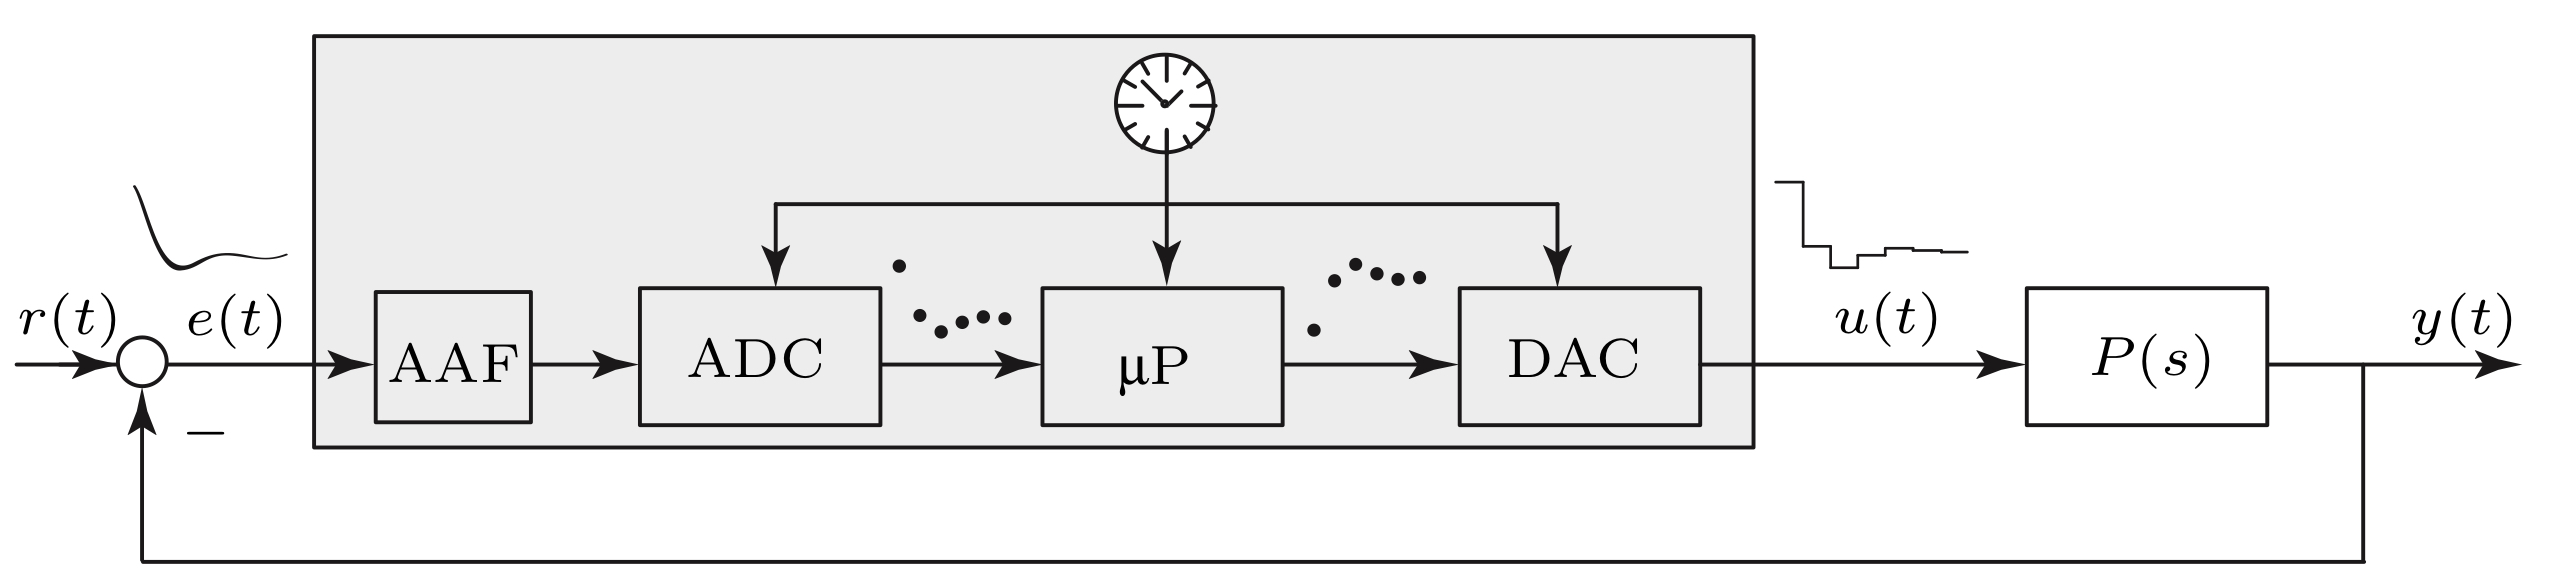
\includegraphics[width = 0.6\linewidth]{images/04/disc_time.jpeg}
        \caption{digitales Regelsystem}
    \end{figure}
    \begin{itemize}
        \item ADC: Analog-to-Digital Converter. Konvertiert zeit-kontinuierliche Signale in zeit-diskrete.
        
        \item $\mu$P: Mikroprozesser. Berechnet zeit-diskreten Eingang $u[k]$.
        
        \item DAC: Digital-to-Analog-Converter Konvertiert zeit-diskrete Signale in zeit-kontinuierliche (meistens ein \textit{Zero-order Hold}).
        \begin{equation*}
            u(t) = u[k] \quad \forall t\in [k\cdot T_s,(k+1)\cdot T_s]
        \end{equation*}
    \end{itemize}
    
    \begin{figure}[H]
        \centering
        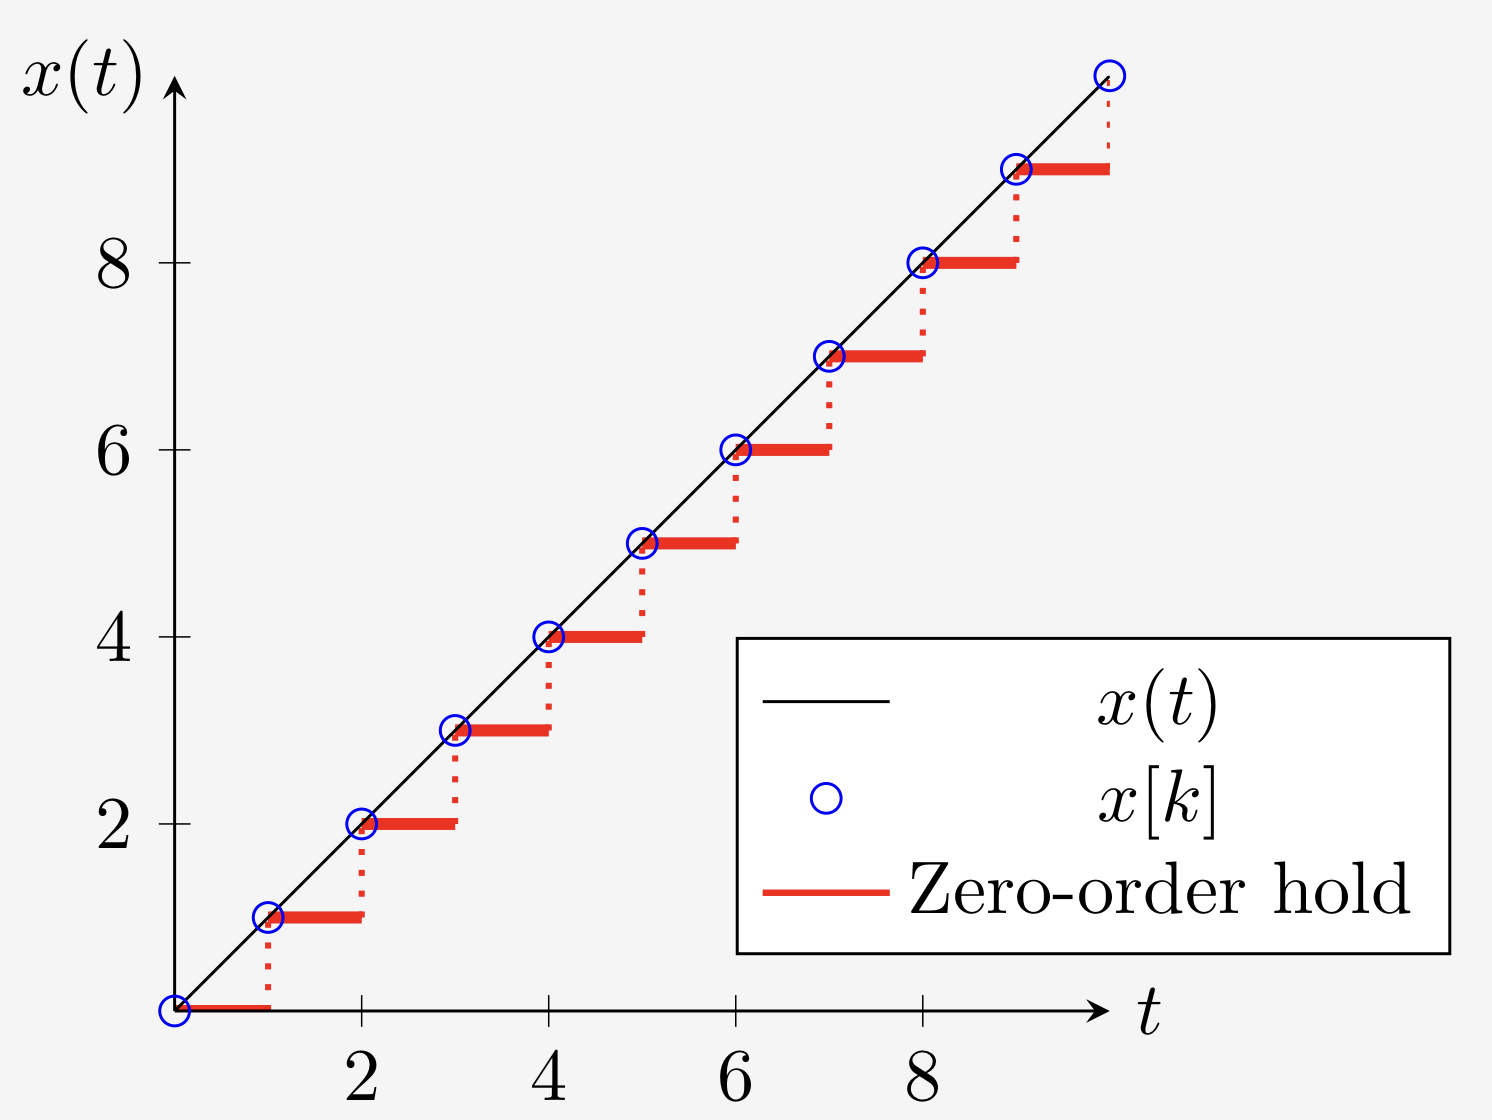
\includegraphics[width = 0.45\linewidth]{images/04/0order_hold.jpeg}
        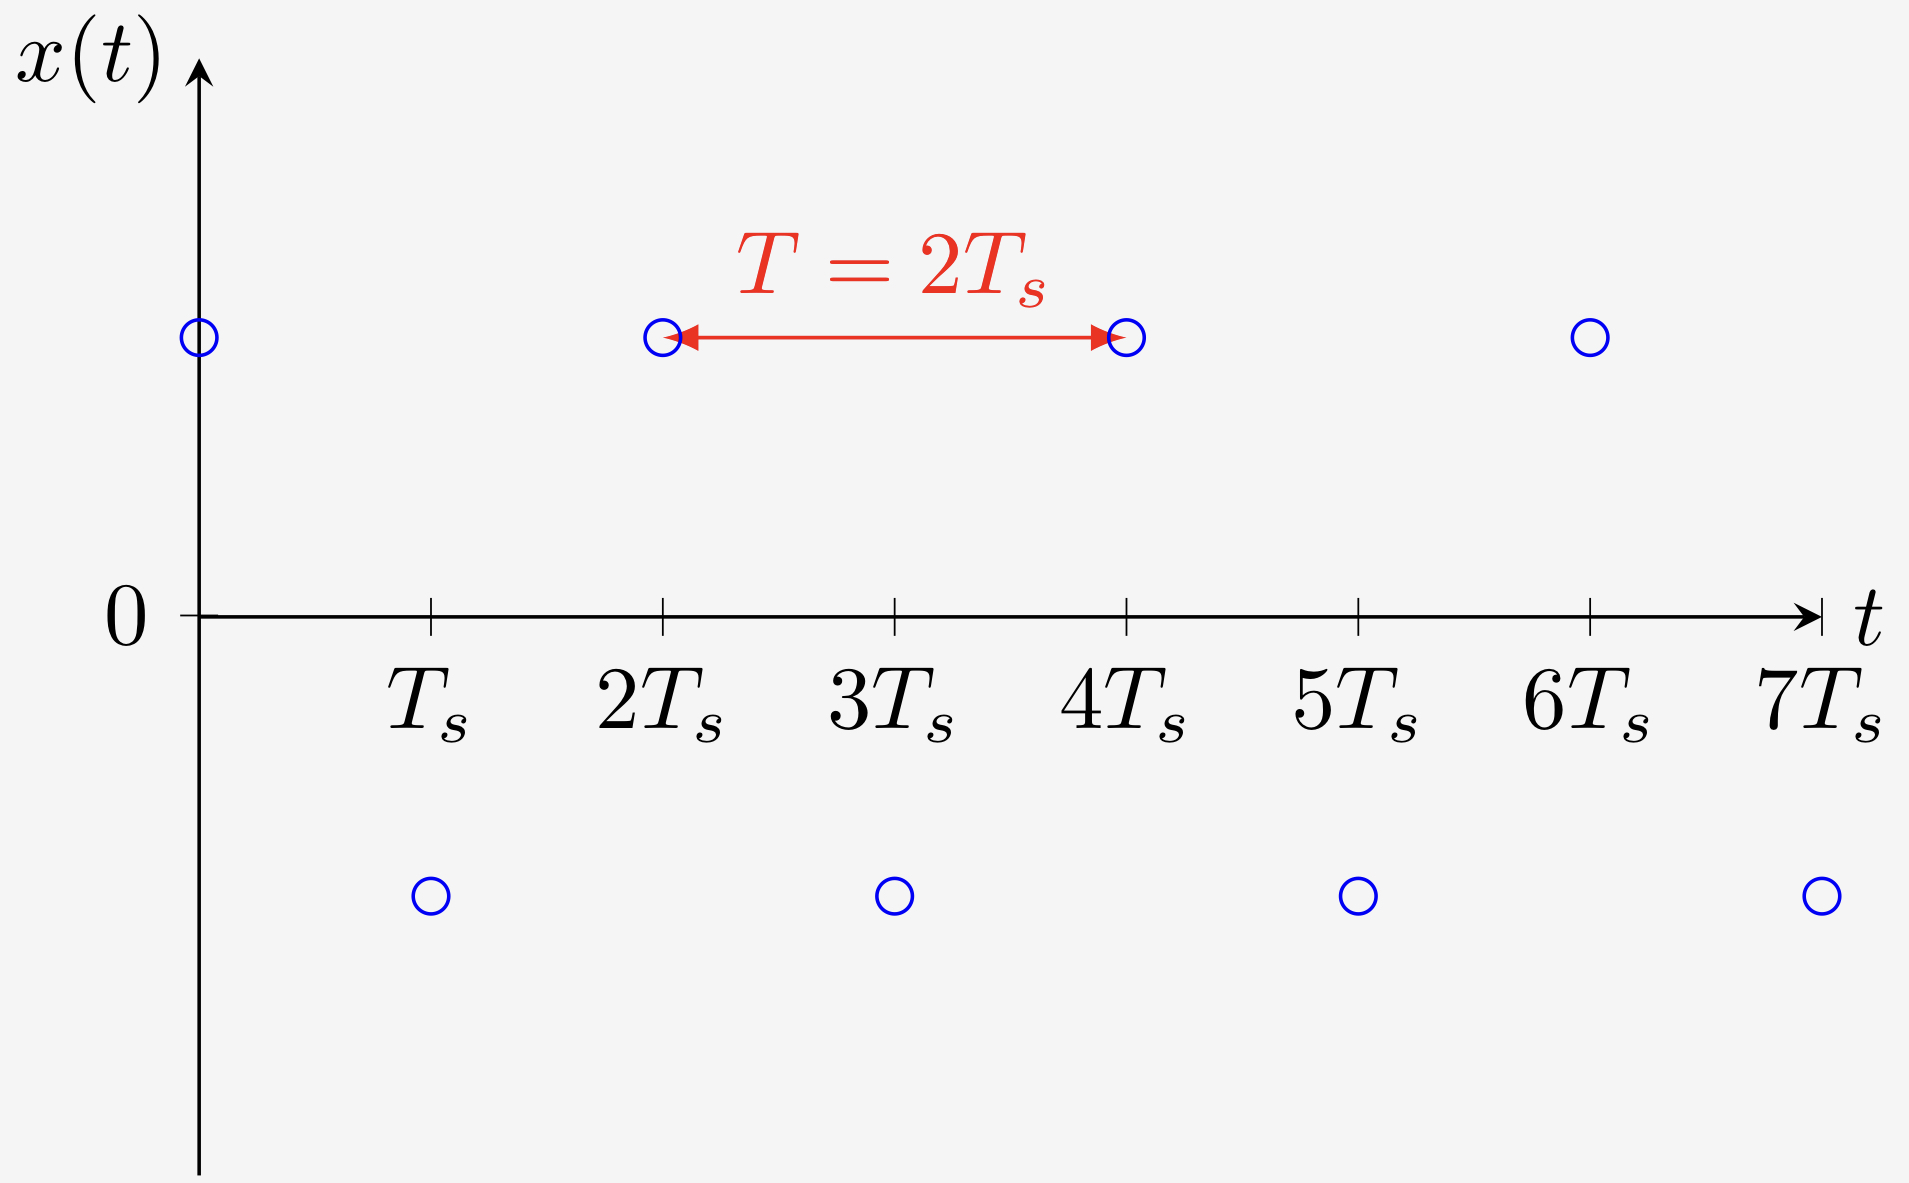
\includegraphics[width = 0.45\linewidth]{images/04/freq_disctime.jpeg}
    \end{figure}
    
    Für eine fixe Rate $\mathit{f}_s = \frac{1}{T_s}$ soll man ein Signal Zeichnen, welches die höchstmögliche Frequenz hat. Die höchstmögliche Frequenz, die man in das Zeitraster $\{0,T_s,\dots\}$ legen kann lautet:
    \begin{equation*}
        \mathit{f}_\textnormal{max} = \frac{1}{T} = \frac{1}{2T_s} \quad \textnormal{(Nyquist Frequenz)}
    \end{equation*}
    
    \subsubsection{Z-Transform}
        \begin{equation*}
            X(z) = \mathbb{Z}\{x(k)\} = \sum_{k=0}^\infty z^{-k}\cdot x(k)
        \end{equation*}
        Eigenschaften:
        \begin{gather*}
            x(k+1) = z\cdot X(z) - z\cdot x(0)\\
            x(k-1) = z^{-1}\cdot X(z)\\
            z = e^{sT_s}
        \end{gather*}
    
    \subsubsection{Emulation}
        Da $z(s)$ nichtlinear ist benutzt man approximationen um einen Regler zu emulieren. Emulationen sind dann sinnvoll, wenn die diskreten Zeitrschritte $T_s$ sehr klein sind im Vergleich zur Systemdynamik.
        \begin{align*}
            z &= e^{sT_s}    &   &\approx 1+sT_s    &   &\Rightarrow s\approx \frac{z-1}{T_s} &   &\textnormal{Euler Forward}\\
            z &= \frac{1}{e^{-sT_s}}    &   &\approx \frac{1}{1-sT_s}    &   &\Rightarrow s\approx \frac{z-1}{zT_s}  &   &\textnormal{Euler Backward}\\
            z &= \frac{e^{sT_s/2}}{e^{-sT_s/2}}    &   &\approx \frac{1+sT_s/2}{1-sT_s/2}    &   &\Rightarrow s\approx \frac{2(z-1)}{T_s(z+1)}  &   &\textnormal{Tustin Emulation}\\
        \end{align*}
        
        Die Tustin emulation ist die am häufigste verwendete emulation, insbesondere weil damit die ganze linke $s$-Halbebene in der $z$-Ebene in einen Kreis mit Radius kleiner eins ($|z|<1$) gemappt wird. D.h. ein stabiles kontinuierliches System resultiert in einem stabilen diskreten System (Stabil in $z \Leftrightarrow |z|<1$). Euler backward erfüllt diese Kriterium auch, Euler backward hingegen nicht. 
        

    
    